\documentclass[12pt]{article}

% --- Configurações de Linguagem e Fontes ---
\usepackage[brazilian]{babel}
\usepackage[utf8]{inputenc}
\usepackage[T1]{fontenc}
\usepackage{booktabs}
\usepackage{tabularx}
% --- Layout e Margens ---
\usepackage[letterpaper,top=2cm,bottom=2cm,left=3cm,right=3cm,marginparwidth=1.75cm]{geometry}

% --- Matemática e Símbolos ---
\usepackage{amsmath}
\usepackage{amsfonts}
\usepackage{amssymb}

% --- Tabelas Avançadas ---
\usepackage{tabularx} % Necessário para o ambiente tabularx
\usepackage{booktabs} % Necessário para \toprule, \midrule e \bottomrule

% --- Elementos Visuais e Cores ---
\usepackage{graphicx}
\usepackage[dvipsnames,svgnames,x11names]{xcolor}
\usepackage[colorlinks=true, allcolors=blue]{hyperref}
\usepackage{graphicx}
\usepackage{subcaption}

% --- Configuração do Quadro de Problema (problembox) ---
\usepackage[most]{tcolorbox}
\newtcolorbox{problembox}{
    colback=gray!5,     % Cor de fundo leve
    colframe=gray!80!black, % Cor da borda
    arc=2pt,            % Arredondamento dos cantos
    boxrule=0.5pt,      % Espessura da borda
    left=10pt, right=10pt, top=10pt, bottom=10pt,
    enhanced,
    breakable           % Permite que a caixa quebre entre páginas se necessário
}

% --- Configuração de Citações Numéricas ---
% O estilo 'unsrt' organiza por ordem de aparecimento [1], [2]...
\bibliographystyle{unsrt}

\title{Otimização Combinatória Aplicada ao Planejamento de Sprints: Um Modelo de Programação Inteira Binária}
\author{Wesley Sant'Anna}

\begin{document}
\maketitle

\begin{abstract}
Your abstract.
\end{abstract}

\section{Introdução}

No cenário contemporâneo de desenvolvimento de software, o \textit{framework} Scrum consolidou-se como a principal referência entre as metodologias ágeis. Sua filosofia fundamenta-se na adaptabilidade, colaboração e entrega contínua de valor \cite{10.1145/3779657.3779668}, características que permitiram sua expansão para além da computação, alcançando diversos ambientes de gestão \cite{gheorghe2020agile}.

Contudo, um dos desafios críticos na execução do Scrum reside no Planejamento da Sprint (\textit{Sprint Planning}): a seleção ideal de itens do Backlog que maximize a entrega de valor ao cliente sem ultrapassar a capacidade técnica da equipe. Esse dilema de seleção transponibiliza o campo da gestão puramente empírica para o domínio da Pesquisa Operacional (PO) \cite{Pinto2019Scrum}.

Sob a ótica da PO, o planejamento de uma iteração pode ser modelado como um problema de otimização combinatória. Nesse sentido, este projeto propõe o enquadramento das características do Scrum no Problema da Mochila (\textit{Knapsack Problem}) \cite{martello1990knapsack}. O objetivo é tratar cada \textit{User Story} como um item a ser alocado em uma "mochila" (a Sprint), onde o peso representa o esforço estimado (pontos ou horas) e a utilidade representa o valor de negócio, buscando-se, assim, a maximização da entrega dentro de um período de tempo predeterminado


\section{Embasamento teórico}

\subsection{Fundamentação teorica}
Apresenta-se, pontanto, a definição segundo \cite{martello1990knapsack} sobre o que é o Problema da Mochila (\textit{Knapsack Problem}) a partir da ótica que um excursionista (hitch-hiker) deseje preencher sua mochila selecionando, dentre vários objetos possíveis, aqueles que lhe proporcionarão o máximo conforto. Esse problema da mochila pode ser formulado matematicamente numerando os objetos de $1$ a $n$ e introduzindo um vetor de variáveis binárias $x_j$ ($j = 1, \ldots, n$) com o seguinte significado:

\[
x_j =
\begin{cases}
1, & \text{se o objeto } j \text{ for selecionado;} \\
0, & \text{caso contrário.}
\end{cases}
\]

Então, se $p_j$ for uma medida do conforto proporcionado pelo objeto $j$, $w_j$ seu tamanho (peso) e $c$ a capacidade da mochila, nosso problema será selecionar, dentre todos os vetores binários $x$ que satisfazem a restrição

\[
\sum_{j=1}^{n} w_j x_j \leq c,
\]

aquele que maximiza a função objetivo

\[
\sum_{j=1}^{n} p_j x_j.
\]

A associação entre o \textbf{Problema da Mochila clássico} e o \textbf{problema de planejamento de sprint} pode ser feita da seguinte forma:

A relação entre os conceitos de otimização combinatória e a gestão de projetos ágeis pode ser visualizada na Tabela \ref{tab:mochila-sprint}. % Aqui você cria a referência automática

\begin{table}[ht]
\centering
\caption{Correspondência entre o Problema da Mochila e o Planejamento de Sprint}
\label{tab:mochila-sprint}
\begin{tabularx}{\textwidth}{lX}
\toprule
\textbf{Problema da Mochila} & \textbf{Planejamento de Sprint} \\
\midrule
Mochila & Sprint \\
Capacidade da mochila ($c$) & Capacidade de trabalho disponível (horas ou pontos) \\
Objeto $j$ & Tarefa (\textit{story}, \textit{bug}, melhoria, etc.) \\
Peso do objeto ($w_j$) & Esforço estimado da tarefa (horas ou \textit{points}) \\
Valor do objeto ($p_j$) & Prioridade ou valor de negócio \\
Variável binária $x_j$ & Decisão de incluir ou não a tarefa no sprint \\
Restrição de capacidade & Limite de horas disponíveis dos desenvolvedores \\
Função objetivo & Maximizar o valor entregue pelo sprint \\
\bottomrule
\end{tabularx}
\end{table}

Em termos matemáticos, a interpretação fica:

\begin{itemize}
    \item Cada tarefa $j$ possui:
    \begin{description}
        \item[$p_j$:] valor (prioridade, impacto ou valor de negócio);
        \item[$w_j$:] esforço (tempo estimado para execução).
    \end{description}

    \item Define-se:
    \[
    x_j =
    \begin{cases}
    1, & \text{se a tarefa } j \text{ for incluída no sprint;} \\
    0, & \text{caso contrário.}
    \end{cases}
    \]
\end{itemize}


O objetivo é selecionar as tarefas que maximizem o valor total entregue:

\[
\max \sum_{j=1}^{n} p_j x_j
\]

respeitando a capacidade disponível:

\[
\sum_{j=1}^{n} w_j x_j \leq c.
\]


No entanto, o projeto proposto avança além do Problema da Mochila tradicional. Enquanto o modelo clássico possui apenas uma mochila, o sprint possui diversos desenvolvedores, cada um com sua própria capacidade. Assim, o problema se aproxima de uma extensão conhecida como \textbf{Problema da Mochila Múltipla} (Multiple Knapsack Problem - MKP) \cite{martello1990knapsack} \cite{arenales2015pesquisa}.

\begin{itemize}
    \item Cada desenvolvedor $i$ corresponde a uma mochila;
    
    \item Cada desenvolvedor possui uma capacidade $c_i$;
    
    \item Uma tarefa deve ser atribuída a exatamente um desenvolvedor habilitado para executá-la;
    
    \item Podem existir dependências entre tarefas;

\end{itemize}

A variável de decisão torna-se:
\[
x_{ij} =
\begin{cases}
1, & \text{se a tarefa } j \text{ for atribuída ao desenvolvedor } i; \\
0, & \text{caso contrário.}
\end{cases}
\]


\subsection{Definição do problema}
Nesse sentido, segue-se a apresentação do problema:


\begin{problembox}
    \color{gray!80!black} % Deixa o texto cinza escuro
    \itshape % Itálico opcional para dar cara de "contexto"
    Considere que um time de desenvolvimento possua um backlog com $n$ tarefas disponíveis para execução, cada uma com um valor de negócio $p_j$ (medido em \textit{story points}) e um esforço estimado $w_j$ (medido em horas). 

O time é composto por $m$ desenvolvedores, cada um com uma capacidade de trabalho $c_i$ (horas disponíveis no sprint). Além disso, nem todo desenvolvedor está habilitado para executar qualquer tarefa — a matriz $s_{ij} \in \{0,1\}$ indica se o desenvolvedor $i$ possui a habilidade necessária para a tarefa $j$. 

Por fim, algumas tarefas possuem dependências: a tarefa $j'$ só pode ser incluída no sprint se a tarefa $j$ também for, conforme indicado pela matriz $d_{jj'} \in \{0,1\}$. O gerente do projeto deve selecionar e atribuir tarefas aos desenvolvedores buscando maximizar o valor de negócio total entregue ao final do sprint, sem exceder a capacidade de trabalho de nenhum desenvolvedor, respeitando as qualificações de cada um e as dependências entre tarefas. Modele matematicamente esse problema como uma extensão do Problema da Mochila Múltipla com restrições de qualificação e precedência, formulada como Programação Inteira Binária.
\end{problembox}


\subsection{Modelagem Matemática}
Segue-se: 
\begin{equation}
\max Z = \sum_{i \in M}\sum_{j \in N} p_j x_{ij}
\end{equation}

sujeito a

\begin{equation}
\sum_{j \in N} w_j x_{ij} \le c_i,
\quad \forall i \in M
\end{equation}

\begin{equation}
\sum_{i \in M} x_{ij} \le 1,
\quad \forall j \in N
\end{equation}

\begin{equation}
x_{ij} \le s_{ij},
\quad \forall i \in M,\; j \in N
\end{equation}

\begin{equation}
\sum_{i \in M} x_{ij'}
\le
\sum_{i \in M} x_{ij},
\quad \forall (j,j') \text{ tais que } d_{jj'} = 1
\end{equation}

\begin{equation}
x_{ij} \in \{0,1\},
\quad \forall i \in M,\; j \in N
\end{equation}

A função objetivo (1) representa a maximização do valor total entregue pelo sprint, somando as prioridades $p_j$ de todas as tarefas $j$ alocadas a cada sprint $i$. As restrições (2) garantem que o esforço total das tarefas alocadas ao sprint $i$ não excede sua capacidade disponível $c_i$, seja em horas ou pontos. As restrições (3) asseguram que cada tarefa $j$ é alocada a no máximo um sprint, evitando duplicidade. As restrições (4) impõem que uma tarefa $j$ só pode ser alocada ao sprint $i$ se tal alocação for permitida pela matriz de elegibilidade $s_{ij}$, contemplando restrições de disponibilidade de equipe ou dependências externas. As restrições (5) modelam dependências de precedência entre tarefas: se a tarefa $j'$ depende da tarefa $j$ (isto é, $d_{jj'} = 1$), então $j'$ somente pode ser alocada a um sprint se $j$ também o for, garantindo que pré-requisitos sejam respeitados. Por fim, a restrição (6) define o domínio binário das variáveis de decisão $x_{ij}$, indicando se a tarefa $j$ é ou não incluída no sprint $i$.

\section{Método de Solução}

Para fundamentar as decisões do \textit{Product Owner} (PO) de forma analítica, aplicamos um modelo de Programação Inteira Binária (BIP) ao cenário prático denominado \textbf{PagaFácil}. O problema consiste na seleção e alocação de itens de um \textit{backlog} para uma \textit{sprint}, considerando restrições de capacidade, qualificação técnica e precedência entre tarefas \cite{wolsey1998}.

% --- TODA A ESTRUTURA DO PAGAFÁCIL EM UMA ÚNICA SUBSECTION ---
\subsection{Cenário Prático 1: O Caso PagaFácil}

% Transformado em subsubseção para não quebrar a regra
\subsubsection{Contextualização do Cenário e Dados do Backlog}

Consideramos uma equipe de $m=2$ desenvolvedores e um \textit{backlog} de $n=3$ tarefas. Os parâmetros de capacidade ($c_i$), espaço ($e_j$) e valor de negócio ($v_j$) são detalhados nas Tabelas \ref{tab:equipe} e \ref{tab:backlog}.

\begin{table}[h]
\centering
\caption{Capacidade e Especialização da Equipe}
\label{tab:equipe}
\begin{tabular}{lllc}
\hline
$i$ & Desenvolvedor & Especialização & $c_i$ (h) \\ \hline
1   & Ana           & Backend (Node.js, PostgreSQL) & 40        \\
2   & Bruno         & Frontend (React Native)       & 28        \\ \hline
\end{tabular}
\end{table}

\begin{table}[h]
\centering
\caption{Backlog da Sprint}
\label{tab:backlog}
\begin{tabular}{llcc}
\hline
$j$ & Descrição & $e_j$ (h) & $v_j$ \\ \hline
1   & T1: Modelagem do schema de usuários & 20        & 20    \\
2   & T2: Endpoints JWT de autenticação   & 26        & 80    \\
3   & T3: Interface de login e recuperação & 22        & 55    \\ \hline
\end{tabular}
\end{table}

A matriz de qualificação $S \in \{0,1\}^{m \times n}$ define que Ana é apta para T1 e T2, enquanto Bruno é apto para T3 \cite{bellenguez2007}:
\[
S = \begin{bmatrix} 1 & 1 & 0 \\ 0 & 0 & 1 \end{bmatrix}
\]

A matriz de dependência $D \in \{0,1\}^{n \times n}$ estabelece que $d_{12}=1$, ou seja, a tarefa T2 exige que T1 também seja selecionada na \textit{sprint} para garantir a integridade técnica do sistema \cite{bagnall2001}.


\subsubsection{Formulação Matemática Aplicada}

O objetivo é maximizar o valor total entregue, respeitando as três famílias de restrições:
\begin{itemize}
    \item \textbf{Capacidade:} $\sum_{j=1}^{n} e_j x_{ij} \leq c_i, \forall i$.
    \item \textbf{Qualificação:} $x_{ij} \leq s_{ij}, \forall i,j$.
    \item \textbf{Precedência:} $\sum_{i=1}^{m} x_{i,jp} \leq \sum_{i=1}^{m} x_{ij}$, onde $d_{j,jp}=1$ \cite{samphaiboon2000}.
\end{itemize}

No cenário PagaFácil, a restrição de capacidade de Ana ($20x_{11} + 26x_{12} \leq 40$) impede a realização simultânea de T1 e T2. Como T2 depende de T1, a tarefa T2 torna-se inviável, alterando o ponto ótimo do planejamento \cite{ruhe2005}.


\subsubsection{Resultados e Validação}

A solução ótima encontrada fixa $x_{11}=1$ (Ana em T1) e $x_{23}=1$ (Bruno em T3), com valor total de 75. A Tabela \ref{tab:validacao} apresenta a análise de sensibilidade através da relaxação de restrições.

\noindent % Garante que o bloco comece alinhado à esquerda
\begin{nopagebreak} % Evita que as imagens se separem entre páginas diferentes
\begin{center}
    % ---- PRIMEIRA LINHA DE IMAGENS ----
    \begin{minipage}{0.48\textwidth}
        \centering
        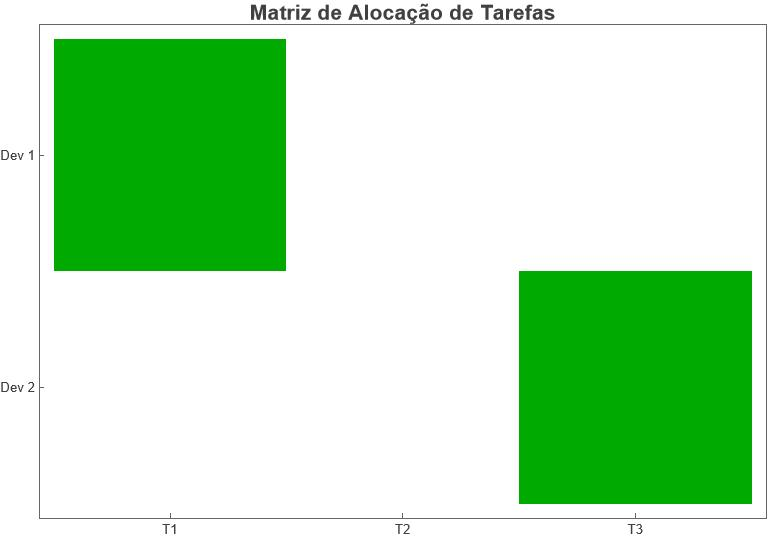
\includegraphics[width=\textwidth]{img/matrizAlocacao.jpg}
        \textsf{\small Imagem 1: Matriz de alocação de tarefas} % Texto simples, não conta em listas
    \end{minipage}
    \hfill % Empurra a próxima imagem para a direita
    \begin{minipage}{0.48\textwidth}
        \centering
        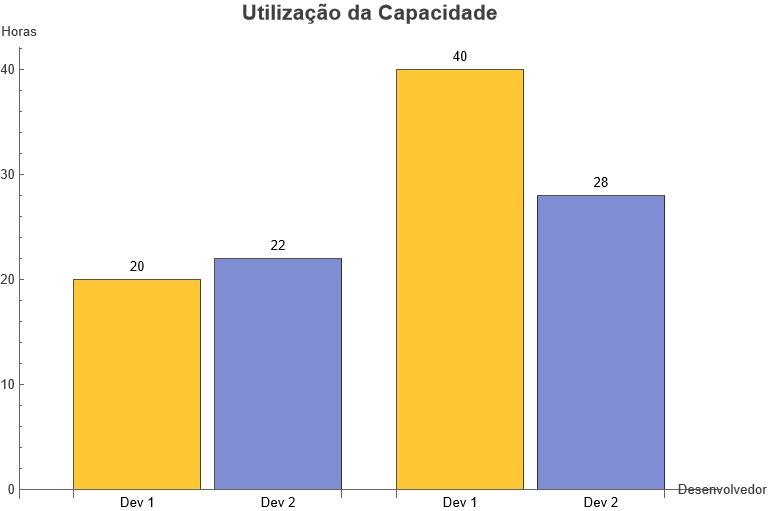
\includegraphics[width=\textwidth]{img/capacidade.jpg}
        \textsf{\small Imagem 2: Utilização da capacidade}
    \end{minipage}
    
    \vspace{0.6cm} % Espaço vertical entre as linhas
    
    % ---- SEGUNDA LINHA DE IMAGENS ----
    \begin{minipage}{0.48\textwidth}
        \centering
        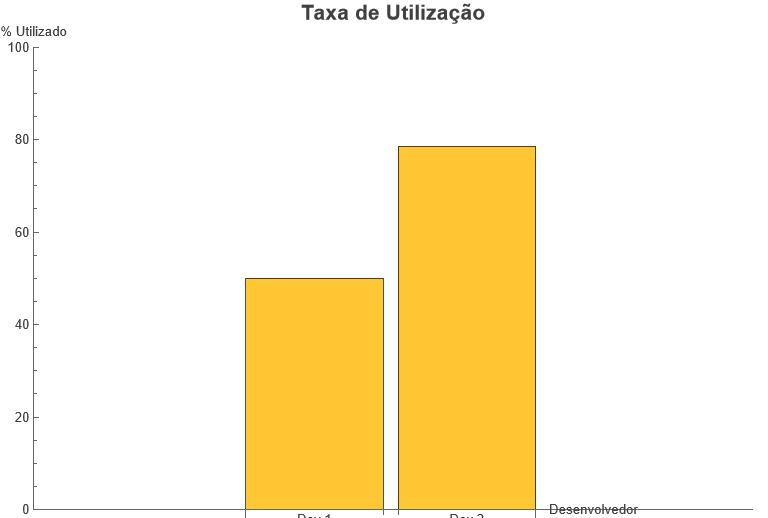
\includegraphics[width=\textwidth]{img/taxaUtilizacao.jpg}
        \textsf{\small Imagem 3: Taxa de utilização}
    \end{minipage}
    \hfill
    \begin{minipage}{0.48\textwidth}
        \centering
        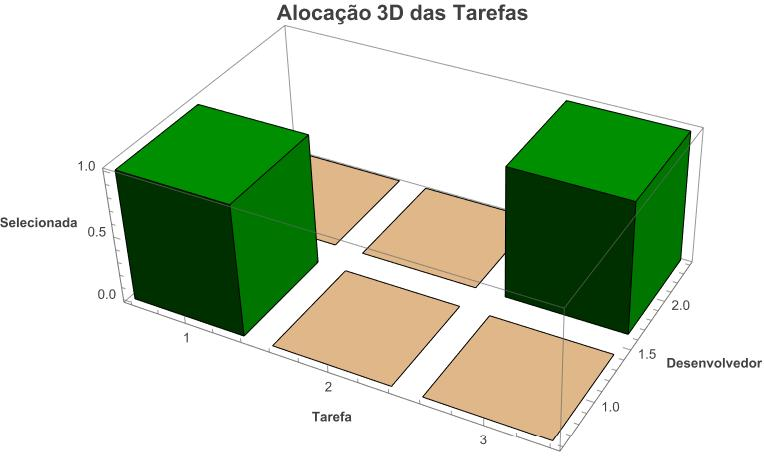
\includegraphics[width=\textwidth]{img/alocacao3D.jpg}
        \textsf{\small Imagem 4: Alocação de tarefa em 3D}
    \end{minipage}
\end{center}
\end{nopagebreak}

\begin{table}[h]
\centering
\caption{Validação por Relaxação de Restrições}
\label{tab:validacao}
\begin{tabular}{llc}
\hline
Restrições Ativas & Solução Ótima & Valor \\ \hline
Todas (cap + qual + dep) & \{T1 $\to$ Ana, T3 $\to$ Bruno\} & 75 \\
Sem precedência ($D=0$) & \{T2 $\to$ Ana, T3 $\to$ Bruno\} & 135 \\
Sem qualificação (com dep) & \{T1 $\to$ Ana, T2 $\to$ Bruno\} & 100 \\
Sem qualif. + sem dep & \{T2 $\to$ Ana, T3 $\to$ Bruno\} & 135 \\ \hline
\end{tabular}
\end{table}

Este modelo, fundamentado no Problema da Mochila Múltipla \cite{kellerer2004}, permite ao PO justificar tecnicamente a exclusão de itens de alto valor (como T2) que, embora desejáveis, são inviáveis dadas as dependências e limitações de capacidade da equipe.

% -----------------------------------------------------------------
% Espaço preparado para o seu próximo cenário de escala maior:
% \subsection{Cenário Prático 2: Cenário Ampliado (Escala Real)}

\section{Experimentos computacionais}

\section{Análise dos Resultados}

\section{Conclusões e trabalhos futuros}



\bibliographystyle{alpha}
\bibliography{sample}

\end{document}
